\documentclass[a4paper]{article}

\usepackage[fontset=fandol]{ctex}
\usepackage{amsmath, amssymb}
\usepackage{graphicx}
\usepackage[margin=2.4cm]{geometry}
\usepackage[most]{tcolorbox}
\usepackage{hyperref}
\usepackage{booktabs}
\usepackage{float}
\usepackage{enumitem}

\newtcolorbox{knowledgebox}[1]{
    enhanced, colback=blue!5!white, colframe=blue!75!black, colbacktitle=blue!75!black,
    coltitle=white, fonttitle=\bfseries, title=#1, attach boxed title to top left={yshift=-2mm, xshift=2mm},
    boxrule=1pt, sharp corners
}

\newtcolorbox{importantbox}[1]{
    enhanced, colback=yellow!10!white, colframe=yellow!80!black, colbacktitle=yellow!80!black,
    coltitle=black, fonttitle=\bfseries, title=#1, sharp corners
}

\newtcolorbox{warningbox}[1]{
    enhanced, colback=red!5!white, colframe=red!75!black, colbacktitle=red!75!black,
    coltitle=white, fonttitle=\bfseries, title=#1, sharp corners
}

\newcommand{\notetitle}{CS294/194-196 第 13 讲：Agentic AI 的安全与安全性}
\newcommand{\noteauthors}{Codex 基于 Dawn Song 直播录播字幕与官方课程页重写}
\newcommand{\notedate}{2026-04-16}
\newcommand{\videourl}{https://youtube.com/live/CvZDJxd4LKM?feature=share}
\newcommand{\videocoverpath}{../../raw/13_CvZDJxd4LKM/13_CvZDJxd4LKM.jpg}

\begin{document}

\begin{titlepage}
\centering
{\Large 课程讲义\par}
\vspace{1.2cm}
{\huge\bfseries \notetitle\par}
\vspace{0.8cm}
{\large \noteauthors\par}
\vspace{0.3cm}
{\large \notedate\par}
\vspace{1.2cm}
\includegraphics[width=0.82\textwidth,height=0.45\textheight,keepaspectratio]{\videocoverpath}\par
\vfill
\begin{tcolorbox}[width=0.9\textwidth, colback=black!2!white, colframe=black!60, sharp corners]
\textbf{课程}：UCB CS294/194-196 Agentic AI（Fall 2025）\par
\textbf{讲次}：Agentic AI Safety \& Security\par
\textbf{主讲}：Dawn Song\par
\textbf{说明}：本讲官方课程页没有提供 slides，正文依据直播录播字幕与课程页信息做 best effort 教材化重建。\par
\textbf{视频}：\href{\videourl}{\nolinkurl{\videourl}}
\end{tcolorbox}
\end{titlepage}

\tableofcontents
\newpage

\section{为什么 agentic AI 的风险在 2025 年被重新放大}
这一讲一开场就给出一个非常鲜明的张力：一方面，2025 被反复描述为 “year of agents”；另一方面，frontier AI 和 agentic AI 的快速增长也让安全（safety）与安全性（security）问题同步放大。Dawn Song 的核心判断是：\textbf{一旦 AI 系统能够在更广泛的环境里自主规划、调用工具、访问外部资源并执行动作，攻击者就会比以往有更强的激励去利用这些系统，而系统失误的后果也会更严重。}

她在开头引用了一份由众多学者参与的国际 AI safety 报告，其作用不是给出某个单点结论，而是说明风险谱系已经非常广，不再只是“模型会不会胡说八道”的层面。对 agentic AI 来说，风险问题从一开始就是系统问题，而不是最后再附加上的 compliance checklist。

\subsection{本章小结}
本讲的出发点不是保守主义，而是现实主义：agent 越强、越接近真实世界任务，攻击和误用的激励就越高，安全讨论也越不能停留在模型层表面。

\section{Safety 与 Security：为什么这两者既不同又分不开}
讲者在 transcript 里给出了一个很适合教材化的区分：\textbf{AI safety} 主要关心系统对外部环境可能造成的伤害，\textbf{AI security} 则主要关心系统本身如何抵御来自外部恶意主体的攻击与利用。这个区分很重要，因为它把两个常被混用的词分离开了。

如果把这两者写成更系统化的表述，可以理解为：
\begin{itemize}[leftmargin=1.5em]
\item \textbf{Safety}：系统是否会以错误、失控或不符合目标的方式作用于世界；
\item \textbf{Security}：系统是否会被恶意输入、恶意环境、恶意工具或恶意用户所利用和操纵。
\end{itemize}

但讲者马上又补了一句更关键的话：它们在 agentic AI 上是分不开的。原因很简单，许多 safety mechanism 本身也必须在 adversarial setting 下成立。例如一个 alignment mechanism 如果在攻击者输入下轻易失效，那它就同时是 safety failure 和 security failure。

\begin{importantbox}{这讲最值得保留的定义}
对 agentic AI 来说，safety 与 security 的关系不是两个平行模块，而是一个相互嵌套的系统问题：系统既要不伤害世界，也要不被恶意世界轻易接管。
\end{importantbox}

\subsection{本章小结}
这讲没有把 safety 和 security 当成两个松散话题，而是明确指出：对 agentic system 来说，它们共享同一个闭环，只是关注方向不同。

\section{为什么 agent 系统的攻击面比单模型更大}
讲者接下来把注意力从 base model 拉到了整套 agent stack。她明确说，LLM 的安全与安全性固然是基础，但 agentic AI 的整体风险远不止模型层。原因在于 agent system 还会加入 perception、reasoning、planning、tool use、retrieval、memory 和 environment interaction。每增加一层能力，攻击面也就增加一层。

\begin{figure}[H]
\centering
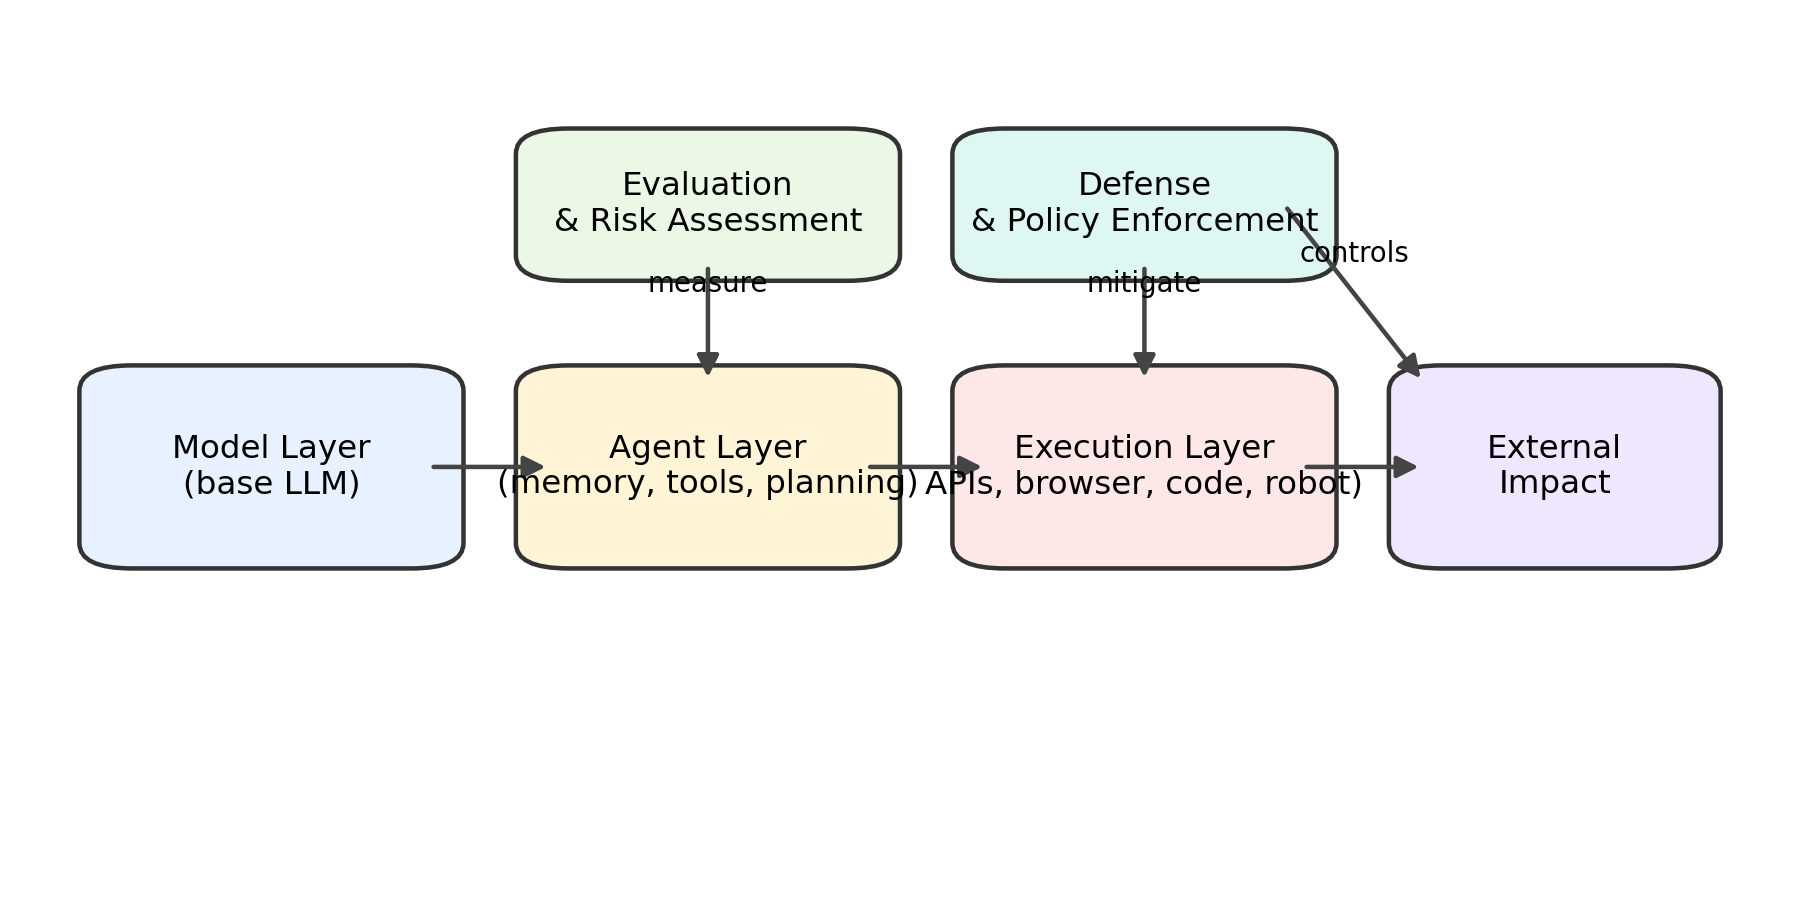
\includegraphics[width=0.88\textwidth]{figures/agentic_safety_layers.png}
\caption{Agentic AI 的分层攻击面：从 base model，到 memory/tool/planning，再到 execution layer 与 external impact。}
\end{figure}

这讲对 agent stack 的直觉可以概括成：模型层的 prompt injection、越狱和 misalignment 只是基础风险；一旦系统允许调用工具、检索外部知识、维护 memory、执行 browser/terminal/robot actions，问题就会升级成完整的 system risk。例如：
\begin{itemize}[leftmargin=1.5em]
\item 工具调用可能被恶意输入诱导；
\item retrieval 结果可能被投毒；
\item memory 可能泄露、污染或被持久化利用；
\item policy enforcement 若不明确，agent 可能越权执行。
\end{itemize}

\begin{warningbox}{为什么 agent 比单模型更脆弱}
一个单纯生成文本的模型，失误通常停留在文本层；一个能调工具、记住历史、执行动作的 agent，失误会沿着 system interface 向外扩散。因此 agent 的风险管理必须从 system boundary 开始设计。
\end{warningbox}

\subsection{本章小结}
agent 的能力增强并不是单调利好。memory、tools、retrieval 和 action 让系统更有用，也让系统更容易被攻击与误用。

\section{评测与风险评估：没有 measurement 就没有安全}
讲者在中段明确说，agentic AI 需要 evaluation 和 risk assessment。这个判断非常关键，因为它把安全讨论从抽象原则拉回到 operational discipline：如果没有稳定的 measurement，你就既无法比较风险，也无法验证 defense 是否有效。

对 agentic system 而言，evaluation 不能只在 model level 进行。至少需要有三层：
\begin{enumerate}[leftmargin=1.5em]
\item \textbf{Model-level evaluation}：base model 在安全、越狱、合规等方面的基础能力；
\item \textbf{System-level evaluation}：memory、tool use、policy、retrieval 和 workflow 组合后的整体行为；
\item \textbf{Adversarial / misuse evaluation}：在攻击者存在的情况下，系统会不会被操控、泄露信息或执行危险动作。
\end{enumerate}

这也解释了为什么 transcript 后半段会反复提到 evaluation、risk assessment、trustworthiness evaluation 和 cyber security benchmark：agent 的安全不能靠“我们觉得它还行”，而要靠明确的测量和持续的 red teaming。

\subsection{为什么 evaluation 会反过来塑造系统设计}
一旦你承认 system-level evaluation 必须存在，就会倒逼系统增加更多可审计结构，例如更清晰的 policy boundary、更可追踪的 action log、更明确的 memory state 和更严格的 tool permission。这一点和课程前面的 evaluation 课完全对齐：\textbf{evaluation 不是最后的打分动作，而是系统设计本身的一部分。}

\subsection{本章小结}
agentic AI 的安全问题无法只靠原则陈述解决，必须转化为可以持续测量、持续回归、持续对抗测试的评估对象。

\section{Defense 与 policy enforcement：如何让 agent 在边界内行动}
讲者在安全栈里特别强调 defenses 与 policy enforcement。这个点很像 enterprise deployment 和 agent evaluation 课的延伸：如果系统没有明确策略边界，它再强也不安全；如果系统有策略边界但不能执行，它也不安全。

从 transcript 可抽象出一条相当明确的工程路线：先定义允许与禁止的动作，再把这些限制落实到 tool invocation、memory access、retrieval scope 和 execution environment 上，最后再用 evaluation 去检验这些限制是否真的生效。也就是说，policy enforcement 不是独立组件，而是嵌在 agent state update 与 action selection 过程里的约束系统。

\begin{knowledgebox}{这讲的 defense 直觉}
最有效的防御通常不是给模型加一句“请安全回答”，而是把 agent 能做什么、能看到什么、什么时候必须停下，写进系统结构本身。
\end{knowledgebox}

\subsection{cyber security 为什么会成为最后的高风险场景}
这讲结尾专门把 cyber security 单列出来，不是偶然。对 agent 而言，cyber security 是最典型的高风险环境：工具丰富、攻击者主动、反馈快速、潜在后果严重，而且模型能力越强，攻击者也越愿意把它当成 leverage。也正因如此，cyber security 对 agentic AI 来说既是应用机会，也是风险放大器。

\subsection{本章小结}
defense 的核心不是抽象口号，而是把策略约束写进系统执行路径。cyber security 则提醒我们：agent 能力一旦进入高对抗环境，安全问题会迅速放大。

\section{总结与延伸}
这讲最值得带走的结论有四点。

第一，\textbf{agentic AI 的风险问题不是 model-only，而是 full-stack system problem。}

第二，\textbf{safety 与 security 可以区分，但对 agent system 来说必须一起设计。}

第三，\textbf{memory、tool use、retrieval、planning 和 execution 会显著扩大攻击面。}

第四，\textbf{真正可靠的防御来自 evaluation、risk assessment 和 policy enforcement 的持续闭环，而不是一次性加固。}

\subsection{本章小结}
Lecture 13 的意义，是把整门 Agentic AI 课程拉回一个现实边界：agent 越接近真实任务执行，越必须在系统层同时考虑安全、攻击、评估和治理。

\end{document}
